\section{Background}
\label{ch:background}

This chapter is separated into two essential parts which contain background
knowledge necessary to understand the problem and methodology used in this 
thesis. As stated in the introduction the goal of this thesis is to apply deep
learning techniques to the prediction of tweet engagement metrics. Therefore,
the first section (ch. 2.1) presents deep learning basics as well as the current
state-of-the-art of research in this area. In the second section (ch. 2.2), 
basics about social networks are established. The section also covers necessary 
Twitter terminology.

\subsection{Deep Learning}
\label{sec:deep_learning}

The application of deep learning techniques has accelerated the progress of 
machine learning (ML) and artificial intelligence (AI) research in recent years~\cite{Brynjolfsson2017}. 
This section aims to explain deep learning from the ground up. Thus, the 
first subsection (ch. 2.1.1) defines basic terminology around this topic 
and before the second (ch. 2.1.2) delivers historical perspectives on deep learning research. 
Basic elements and algorithms used in deep neural networks are explained in the third 
subsection (ch. 2.1.3), before recent developments in research are
presented (ch. 2.1.4). The last subsection (ch. 2.1.5) describes how
deep learning models are applied in practice.

\subsection{Terminology}
\label{sub:dl_terminology}

% AI, ML & DL confusion
In order to understand the concepts behind deep learning, the term has to be
separated from already mentioned areas machine learning and artificial
intelligence, as well as also common term \textit{neural networks}. 
These terms are often used interchangeably, but each defines a distinct area of 
research and they essentially mean different things.
\textbf{Artificial intelligence (AI)} is a research area that aims to understand
and build intelligent entities (often called \textit{agents}). Hence, AI touches the 
areas of philosophy, mathematics, psychology and computer science. Here, 
intelligence is defined as \textit{rational action}, which means that an agent aims
to perform the best possible action in a given setting~\cite{Russell1995}.

In order to perform actions in an intelligent mannner, agents need to be able
to recognize patterns in observed data. The found patterns can then be used
by the agent to build up knowledge. This process is known as \textbf{machine
learning (ML)}~\cite{Goodfellow2016}. In order to understand the methodology in
later chapters of this thesis, a more detailed examination of machine learning
problems is needed. Mitchell~\cite[p. 2]{Mitchell1997} offers the following 
definition for machine learning algorithms:

\begin{quote}
  A computer program is said to learn from experience E with respect to some
  class of tasks T and performance measure P, if its performance at tasks in T,
  as measured by P, improves with experience E.
\end{quote}

Following this definition, a machine learning algorithm can be classified along
three dimensions. Below, these dimensions are explained using the running
example of an algorithm that aims to predict house prices from advertisement data.
Such data might include the number of bedrooms, square footage and whether
the house includes a garage. Figure~\ref{fig:ml_classification} serves as an orientation and summary for
following remarks.

\begin{figure}[h]
  \centering
  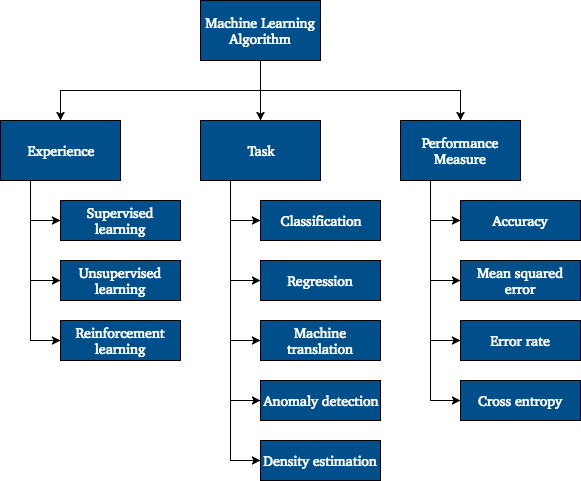
\includegraphics[height=10cm]{img/ml_classification}
  \caption{Classification dimensions of machine learning algorithms}
\label{fig:ml_classification}
\end{figure}

\paragraph{Task \textit{T}}

Machine learning is often used in settings where programs with fixed rules are
insufficient. Hence, the application of machine learning adds a more dynamic
component in order to perform a given task. Here, the task is usually to process
an \textit{example} which consists of a set of \textit{features}. Features are
attributes of an object that can be measured quantitatively~\cite{Goodfellow2016}. 
In the example described above, the number of bedrooms is one the features of 
the house object. The task \textit{T} would then be to predict a price for this 
house. Depending on the type of the specific output variable this problem can 
be assigned to one of many groups of tasks (see Fig.~\ref{fig:ml_classification}). If the output was an
exact price (e.g. 1,000,000\$), this would constitute a \textbf{regression} task. 
Assuming the goal is to assign the house to a price interval (e.g., (500,000\$, 1,000,000\$]),
one would describe this as a \textbf{classification} problem. Other common tasks
can be derived from Figure 2.1. One such example would be \textbf{anomaly detection}, e.g.,
if the goal were to detect expensive houses in a neighborhood where house prices
are typically low. The task could also be to translate house descriptions from
English into other languages (\textbf{machine translation}) or to derive an
estimation of the underlying probability distribution of the data (\textbf{density estimation}).

\paragraph{Performance measure \textit{P}}

In order to perform a task \textit{T} better over time, the algorithm needs
a quantitative measure for its current performance. In the setting of
house price prediction, the algorithm should get feedback on the quality of its
predictions. For a regression problem a suitable performance measure would be 
the \textbf{mean squared error} over all training examples. Possible measures
for classification tasks would be \textbf{accuracy} (i.e., how many examples
were classified correctly?) or the \textbf{error rate} (i.e., how many
examples were classified incorrectly?). If the algorithm outputs class 
probabilities, \textbf{cross entropy} can be used to evaluate model
performance. Defining the correct performance measure can be more difficult
for more complex learning problems such as machine translation. The design of 
\textit{P} can influence the training process, e.g., if not all errors have the
same misclassification cost. Furthermore, machine learning models should be evaluated on unseen
data, i.e., data points that were not used for training the model. This way,
one derives a better estimate of the generalization abilities of the model~\cite{Bishop2006, Goodfellow2016, Mitchell1997}.

\paragraph{Experience \textit{E}}

Machine learning algorithms can further be classified by the `kind of experience
they are allowed to have during the training process'~\cite[p. 104]{Goodfellow2016}.
In \textbf{unsupervised learning} settings the label for an example (also called
\textit{data point}) is unknown. For the house price prediction example this
would mean that real prices for the houses in the data set are not
available for training. Performing classification or regression tasks would
therefore not be feasible as the performance measure \textit{P} can not be
determined. Potential tasks in such an unsupervised learning setting would be
clustering (e.g., identifying similar houses), or performing density estimation
(e.g., to derive the probability for a given house price). In a broad sense these
kinds of algorithms aim to identify underlying distributions of data. Contrary, in 
\textbf{supervised learning} settings each example is associated with an 
observed output (usually called \textit{label} or \textit{target}). Hence, a
performance measure can be calculated for each data point, by which the
algorithm is able to improve its predictions over time (see above classification
and regression examples)~\cite{Goodfellow2016, Bishop2006}. The third kind of
experience for a machine learning algorithm is a \textbf{reinforcement learning}
setting. Here, the algorithm does not rely on a fixed data set, but instead 
interacts with its environment steadily. It then learns from the feedback it
derives from these interactions. A common usecase for reinforcement
learning is the interaction of agents with the real environments, e.g.,
self-driving cars. In most of these settings collecting all data points is
insufficient or simply not feasible~\cite{Sutton1998}.

It becomes obvious that the three dimesions are related, i.e., choices for a
specific dimension are conditioned on the other dimensions. Prior identification 
of all three dimensions is key in order to identify 
`well-defined learning problems'~\cite[p. 2f.]{Mitchell1997}. All developed 
learning algorithms in later chapters will also use this classification 
framework. 


\subsection{History}
\label{sub:dl_history}

After establishing the basic terminology for this thesis, 
it is now possible to take a closer look at the algorithm group of 
\textit{neural networks}. Therefore, this subsection will focus on historical
developments of neural networks, a group of algorithms that deep learning falls
into.
Understanding the origins of this methodology will be helpful in the next 
subsection which explains the more formal aspects of neural networks.
Overall, the history of neural network research is often separated into three
distinct phases of active research and progress in the literature~\cite{Goodfellow2016}.
All three phases will be described in the following.

\paragraph{Phase 1: First models}

The first forms of neural networks were developed in the 1940s, when
researchers tried to model learning machines inspired by the human brain.
The first such model was the McCulloch-Pitts neuron which constituted a linear
model:

\begin{equation}
  f (x, w) = w_1 x_1 + w_2 x_2 + \cdots + w_m x_m
\end{equation}

The neuron was able to recognize two different categories by determining
whether $f(x, w)$ was positive or negative~\cite{McCulloch1943}.
As a downside, there was no way to set the weights via an algorithm.
Instead, the weights had to be set by a human.
The first model of a neuron which overcame this obstacle was the \textit{perceptron}
developed by Rosenblatt~\cite{Rosenblatt1958}. The main contribution of the
perceptron was a simple algorithm to update weights iteratively.
The only requirement for the algorithm to run was a set of labeled examples.
In the same timespan, Widrow and Hoff~\cite{Widrow1960} came up with a similar
model called \textit{adaptive linear element (ADALINE)} for regression problems.
The main disadvantage that could not be overcome at the time lied in the 
linearity of the model which limited its representational capability.
For example, the model from equation 2.1 is not able to learn the XOR function 
(see equations 2.2 to 2.5)~\cite{Minsky1969}.

\begin{align}
  f ([0, 1], w) = 1\\
  f ([1, 0], w) = 1\\
  f ([0, 0], w) = 0\\
  f ([1, 1], w) = 0
\end{align}

These limitations caused a decline in research interest and thus mark the end
of the first phase of neural network research, which is often referred to
as \textbf{cybernetics}~\cite{Goodfellow2016}.

\paragraph{Phase 2: Backpropagation and connectionism}

The second wave of neural network research largely took place from the late
1970s until the mid-1990s. 
The problem of limited representational capability was overcome by wrapping
neurons inside a non-linear function, which basically transforms its output~\cite{Fukushima1975}.
This idea was combined with distributing the representational capacity over
more neurons, thus creating the first \textit{neural networks}. 
The neurons were combined in layers which were connected to each other.
This is also the main reason why this phase of neural network research is
often referred to as \textbf{connectionism}~\cite{Goodfellow2016}.
The intuition behind this was that more neurons would be more capable of
representing the input by acting together. 
Here, each neuron stands for a distinct feature, e.g., the color of an object
or the type of object itself~\cite{Rumelhart1986a}.
Training these more complex models became easier and faster with the
introduction of the backpropagation algorithm~\cite{Rumelhart1986}.
More complex neural networks meant more weights which needed to be updated
iteratively. 
The backpropagation algorithm is still the dominant approach for training
neural networks, because it offers a way of efficiently calculating the
updated weights.
The algorithm will be explained in more detail in the following subsection.
Despite the fast progress in academic research, the interest in neural networks
once again declined in the mid-1990s. The main reasons for this were the
lack of computational power to train deeper models containing more layers, as 
well as the advancements of other fields of machine learning (e.g., Support
Vector Machines) around this time~\cite{Goodfellow2016}.

% Third wave ("deep learning"):
% Training deep networks becomes efficient (Hinton 2006)
% Applications in many areas become possible (to be continued in Recent Developments)

\paragraph{Phase 3: Deep learning}

The difficulties of training deeper neural networks were overcome in 2006.
It was shown that a combination of more efficient training algorithms and
more advanced hardware enabled training deep networks in a reasonable amount of 
time~\cite{Hinton2006, Holden2006}.
Further developments in the techniques and availability of more computational
power led to popularization of deep neural networks and the term \textbf{deep
learning} was coined~\cite{Goodfellow2016, LeCun2015}.
Deep learning was used in models that outperformed other machine learning
algorithms in areas like image and speech recognition~\cite{Krizhevsky2012, Hinton2012}. 
These made use of neural network architectures like \textit{convolutional neural networks} 
and \textit{recurrent neural networks}, that were originally developed during 
the second wave of neural network research~\cite{Fukushima1980, Hochreiter1997, LeCun1998}.

Subsection 2.1.4 will go into more detail about the recent developments of
deep learning techniques. The following subsection will describe the basic
structure, elements and algorithms of neural network architectures in more
detail. This will ease the understanding of the more modern and complex
architectures and lay a mathematical foundation for the later chapters.


\subsubsection{Basic Concepts}
\label{sub:dl_concepts}

Understanding more sophisticated deep learning methods used in later
chapters requires comprehension of the basic concepts behind artificial
neural networks.
This chapter introduces mathematical foundations of both neural network
structure and algorithms.
The notation mostly follows the one from Nielsen~\cite{Nielsen2015}, but also
adds explanations from Bishop~\cite{Bishop2006} and Goodfellow et al.~\cite{Goodfellow2016}.
The first paragraph in this subsection will introduce the major elements
of the neural network training process which will then be described in more
detail in the following paragraphs.

\paragraph{Training process}

Like most machine learning algorithms, neural networks are trained using an iterative process.
In short, the network takes some example from the training data set as an input 
and calculates the respective output via a process called 
\textbf{forward propagation}.
Depending on the size of the data set, it repeats this procedure for more 
examples.
Since this constitutes a supervised learning problem, desired outputs for
each example are known.
These can be used to calculate the prediction error, which is determined by the
\textbf{cost function}.
The assessed error can then be used to calculate updates for the parameters of
the networks which are called \textit{weights}.
This process is known as \textbf{backpropagation}.
The examples which are used during one iteration of the training process are
called a \textit{mini-batch}.
A full run through all examples of the training data set is referred to as an
\textit{epoch}.
The forward and backpropagation algorithms and the cost function are the three
basic elements of an artifical neural network. 
In order to define them in more detail, mathematical notation has first to be
established.

\paragraph{Neural network structure}

\begin{figure}[h]
  \centering
  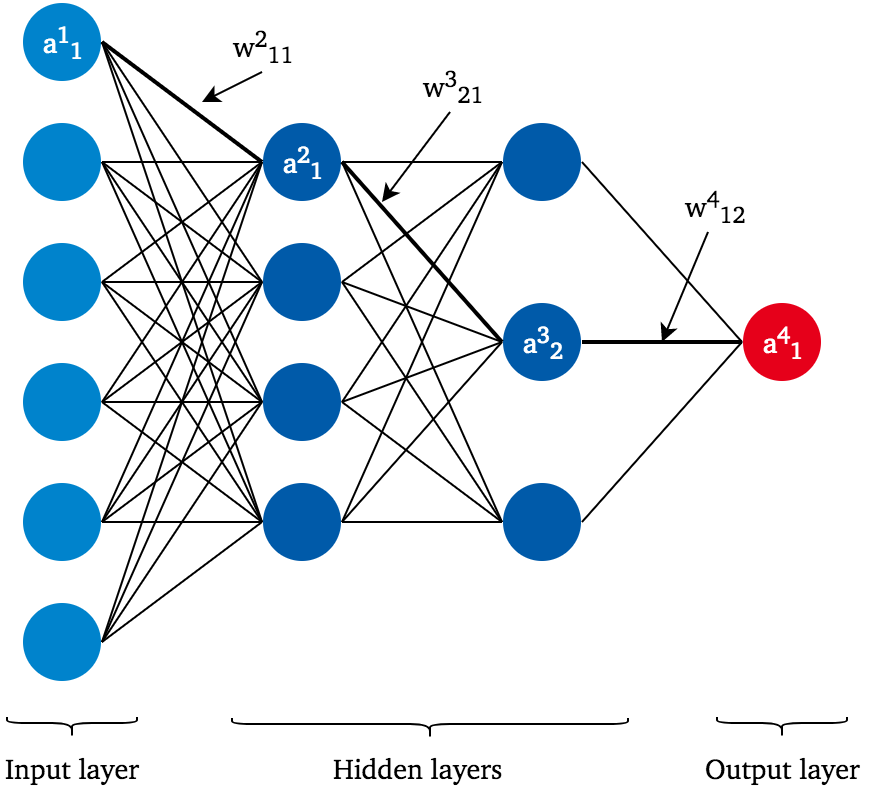
\includegraphics[height=10cm]{img/nn_architecture_2}
  \caption{Neural network structure and notation}
\label{fig:nn_architecture}
\end{figure}

Neural networks basically consist of nodes (also called \textbf{units}) which
are organized as layers.
The single layers of a neural network are wired together via edges that are
called \textbf{weights}.
This subsection will focus on the most basic architecture of a neural network,
called a \textbf{feed-forward network}.
In this architecture all units in a specific layer are connected to all units
in the following layer.
Such a layer is then referred to as being \textit{fully-connected}.
More sophisticated layer architectures will be introduced in subsection~\ref{sub:dl_developments}.
Figure~\ref{fig:nn_architecture} shows an example of a fully-connected network
that contains an input layer with six units, two hidden layers with four respective
three units and and an output layer containing one single unit.
Here, hidden layers are all layers between input and output layer.

In the following, $a_j^l$ will refer to the $j^{th}$ unit in the $l^{th}$ layer.
Weight $w_{jk}^l$ then stands for the weight which connects the $k^{th}$ unit in
the ${(l-1)}^{th}$ layer with the $j^{th}$ unit in the $l^{th}$ layer.
Figure~\ref{fig:nn_architecture} contains an example path from input to ouput
layer which resembles this notation.

\paragraph{Forward propagation}
\label{sub:dl_forward}

During the forward propagation process, the neural network calculates an output
for a specific input with respect to the current weights in the network.
Thus, the network can be written as a function $f(x,w)$ where $x$ is an input
vector or matrix and $w$ is the set of all weights for this network.
The units in the input layer receive their value from the input vector.
All units in later layers are calculated using equation~\ref{eq:activation}.

\begin{equation}
  \label{eq:activation}
  a_j^l = \sigma(\sum_k w_{jk}^l a_k^{l-1} + b_j^l)
\end{equation}

In this equation, $a_j^l$ is also called an \textbf{activation}, $\sigma$ is a
non-linear transformation function and $b_j^l$ is an added bias term.
The bias term is here independent of the activations in the previous layer.
In practice, this calculation can be parallelized for all activations in a layer
by rewriting it in matrix form (see equation~\ref{eq:activation_matrix}).

\begin{equation}
  \label{eq:activation_matrix}
  a^l = \sigma(w^l a^{l-1} + b^l)
\end{equation}

Here, $a^l$ is the vector of all activations in layer $l$, $b^l$ is the vector
of all bias terms in layer $l$ and $a^{l-1}$ is the vector of all activations
in the previous layer. The matrix $w^l$ resembles all connections from layer $(l-1)$
to layer $l$, where $w^l_{jk}$ is the entry in the $j^{th}$ row and $k^{th}$ column.
The function $\sigma$ is applied element-wise to the result vector.

%\outline{What are examples for non-linearities?}
\begin{figure}[h]
  \centering
  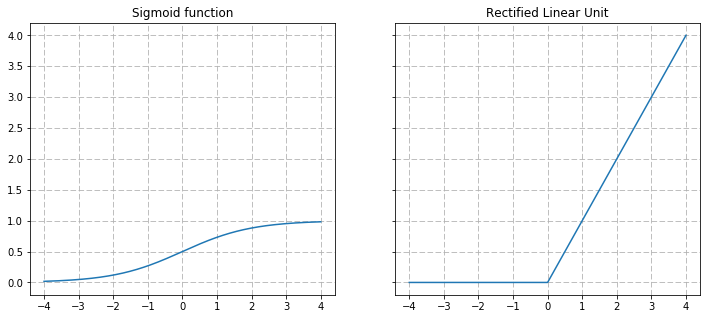
\includegraphics[height=7cm]{img/nn_activations}
  \caption{Popular neural network activation functions}
\label{fig:activations}
\end{figure}

If $\sigma(x) = x$, then the output activations $a^l$ will just be a linear
combination of the input activations $a^{l-1}$.
This property does obviously not change when applied over more layers.
The result will still be a linear function.
In contrast to that, if $\sigma$ is a non-linear function, the network receives more 
representational capability, i.e., it can learn to represent a bigger variety of 
functions. 
Two popular choices for $\sigma$ are the \textit{sigmoid function} and the
\textit{Rectified Linear Unit (ReLU)} (see figure~\ref{fig:activations}). 
The sigmoid function is given by equation~\ref{eq:sigmoid}, whereas ReLU is 
simply equal to the maximum of the input and zero (equation~\ref{eq:relu}).

\begin{equation}
  \label{eq:sigmoid}
  \sigma(x) = \frac{1}{1 + \exp(-x)}
\end{equation}

\begin{equation}
  \label{eq:relu}
  \sigma(x) = \max(0, x)
\end{equation}

Outputs of the sigmoid function are guaranteed to be between zero and one, which fits
the problem of predicting class probabilities.
Hence, the sigmoid function is most commonly applied in output layers of networks that
train on a classification task.
Contrary, most hidden layers in modern neural networks use ReLU as an activation
function.
The function was introduced in 2000 and has shown to be suitable for most deep
learning techniques, since it stabilizes the training process~\cite{Hahnioser2000, Nair2010}.

All in all, forward propagation is the layer-wise application of above described
calculations. For the example network in figure~\ref{fig:nn_architecture}, the
output for an example data point $x$ can be determined according to equation~\ref{eq:forward_prop}.
The enumerator in $\sigma$ indicates that different activation functions can
be applied in each layer.

\begin{equation}
  \label{eq:forward_prop}
  a^4 = \sigma^4(w^4 \sigma^3(w^3 \sigma^2(w^2 x + b^2) + b^3) + b^4)
\end{equation}

With the calculated outputs it is possible to evaluate predictions of the
networks by calculating the error according to the cost function.

\paragraph{Cost function}

In order to state necessary assumptions about the cost function, a first look
at the goal of the backpropagation algorithm is useful.
Backpropagation aims at deriving updates for all weights and biases in
the network.
It does so by calculating the gradients $\partial C / \partial w$ and 
$\partial C / \partial b$ of the cost function with respect to weights and
biases.
Two assumptions about the cost function have to be made, so that the 
backpropagation algorithm is able to work. 
The reasons for these assumptions will be explained in the next paragraph.
For illustration purposes this paragraph will use the \textit{quadratic cost function}
as a running example (see equation~\ref{eq:quad_costs}).
Here, $y(x)$ is the desired output for input $x$, $n$ resembles the number of
examples in the current mini-batch and $L$ denotes the output layer of the
network.

\begin{equation}
  \label{eq:quad_costs}
  C = \frac{1}{2n} \sum_x \Vert y(x) - a^L(x) \Vert^2
\end{equation}

The first assumption (equation~\ref{eq:cost_assump_1}) is that the cost function 
can be calculated as the average of all error terms for the current batch
of training examples. For example the quadratic cost function can be written in
this form, because $C_x = \frac{1}{2} \Vert y - a^L \Vert^2$.

\begin{equation}
  \label{eq:cost_assump_1}
  C = \frac{1}{n} \sum_x C_x
\end{equation}

Secondly, the cost function has to be a function of the network output $a^L(x)$
(see equation~\ref{eq:cost_assump_2}).
Obviously, this is given for the quadratic cost function since $a^L(x)$ is used
for determining the error and all other components are fixed parameters.

\begin{equation}
  \label{eq:cost_assump_2}
  C = C(a^L)
\end{equation}

With these assumptions set the next paragraph will explain how the
backpropagation algorithm derives gradients for the weight updates which enable
learning in the training process.

\paragraph{Backpropagation}
\label{sub:backprop}

As mentioned before, the backpropagation offers a way to calculate gradients
of the cost function with regard to weights and biases of the network.
Optimization algorithms such as gradient descent then make use of these 
gradients when determining weight updates since they intuitively represent
the rate of change of the cost function with respect to these learnable weights.
This paragraph will explain how the backpropagation algorithm works in detail.
Proofs are out of scope for this thesis and therefore omitted completely.

Some definitions are helpful for the further explanations. Firstly
$z^l$ is defined as an intermediate quantity which represents the weighted
inputs for neurons in layer $l$ (see equation~\ref{eq:weighted_input}).

\begin{equation}
  \label{eq:weighted_input}
  z^l \equiv w^l a^{l-1} + b^l \Rightarrow a^l = \sigma(z^l)
\end{equation}

Another useful intermediate quantity is $\delta_j^l$ which denotes the error
in the $j^{th}$ neuron in the $l^{th}$ layer. The error is defined in
equation~\ref{eq:neuron_error} as the partial gradient of the cost function
with respect to the weighted input to the neuron. Intuitively, if this value
is large (positively or negatively), the cost can be lowered by updating the 
weighted input in the opposite direction.

\begin{equation}
  \label{eq:neuron_error}
  \delta_j^l \equiv \frac{\partial C}{\partial z_j^l}
\end{equation}

The following explanation of the backpropagation algorithm is centered around
the four fundamental equations mentioned by Nielsen~\cite{Nielsen2015}.
Since the value of the cost function is known after the forward propagation
procedure, the first step of backpropagation is to calculate the error in the
output layer $L$.
Equation~\ref{eq:bp_1_comp} states how this is achieved for a single neuron,
whereas equation~\ref{eq:bp_1_mat} shows the matrix-based form for efficient
computation in practice. In this equation $\nabla_a C$ is the vector of all partial
derivatives $\partial C / \partial a_j^L$ and $\odot$ denotes the element-wise
multiplication of two vectors, known as the \textit{Hadamard product}.
For the previously introduced quadratic cost function, it would simply hold
that $\nabla_a C = (a^L -y)$.
This is also where the assumption about the cost function as a function of the
output activations $a^L$ comes into play.

\begin{equation}
  \label{eq:bp_1_comp}
  \delta_j^L = \frac{\partial C}{\partial a_j^L} \sigma'(z_j^L)
\end{equation}

\begin{equation}
  \label{eq:bp_1_mat}
  \delta^L = \nabla_a C \odot \sigma'(z^L)
\end{equation}

The expresssions can be split into two components. On the one hand, the partial
derivative represents the rate of change of the cost function with respect to
the output activations, on the other hand $\sigma'(z^L)$ determines how
fast the activation function changes for the weighted input.

After the error in the output layer is calculated, the next logical step is to
compute error terms for the previous layers.
In order to do that, the backpropagation algorithm only requires the error in
the next layer (see equation~\ref{eq:bp_2}).

\begin{equation}
  \label{eq:bp_2}
  \delta^l = ({(w^{l+1})}^T \delta^{l+1}) \odot \sigma'(z^l)
\end{equation}

The basic intuition behind this equation is that the known error $\delta^{l+1}$
flows backward through the network by multiplying it with the weight
matrix $w^{l+1}$.
It is then further moved through the activations of neurons in layer $l$ by
building the Hadamard product with the derivative of the activation function.
In summary, the first two equations offer a way to determine the errors for all
layers in the network.
The final two steps now aim to relate the errors to the partial derivatives
$\partial C / \partial w$ and $\partial C / \partial b$.

Equation~\ref{eq:bp_3} shows that the gradient of the cost function with respect
to any bias in the network is equal to the error at that neuron.
In short, this is also written as stated in equation~\ref{eq:bp_3_short}.

\begin{equation}
  \label{eq:bp_3}
  \frac{\partial C}{\partial b_j^l} = \delta_j^l
\end{equation}

\begin{equation}
  \label{eq:bp_3_short}
  \frac{\partial C}{\partial b} = \delta
\end{equation}

For weights, this computation is slightly more complex because they represent
a connection between two neurons.
In order to derive the gradient for a weight, the error in the current layer
has to be multiplied by the activation of the connected neuron in the previous
layer (see equation~\ref{eq:bp_4}).
This implies that weight updates are smaller if the input activation is near
zero.
Hence, the weight is said to \textit{learn slowly}.

\begin{equation}
  \label{eq:bp_4}
  \frac{\partial C}{\partial w_{jk}^l} = a_k^{l-1} \delta_j^l
\end{equation}

Optimization algorithms make use of the computed gradients in that they determine
updates for all weights and biases in the network.
Figure~\ref{fig:grad_desc} illustrates mechanics of most optimization
algorithms used in neural networks.
Here, a common practice is to use mini-batches, i.e., small collections of
examples, for each iteration of the algorithm.
For each example the output of the network is calculated, which is then used
to determine the output error. 
The error in the output layer is then propagated through the network in order
to compute the gradients for weights and biases.
In the final step of the iteration, the weights (including biases) are updated
according to the gradients.
The most basic optimization algorithm called \textbf{gradient descent} uses the
update formula in equations~\ref{eq:gd_update_weights} and~\ref{eq:gd_update_biases}.

\begin{equation}
  \label{eq:gd_update_weights}
  w^l \rightarrow w^l - \frac{\eta}{m} \sum_x \delta^{x,l}{(a^{x,l-1})}^T
\end{equation}

\begin{equation}
  \label{eq:gd_update_biases}
  b^l \rightarrow b^l - \frac{\eta}{m} \sum_x \delta^{x,l}
\end{equation}

It averages over the gradients determined by looking at single examples, which
is only possible through the first assumption about the cost function (see equation~\ref{eq:cost_assump_1}).
Here, $m$ is the number of examples in the batch and $\eta$ resembles the
\textit{learning rate} which is a hyperparameter that has to be set prior to
learning.

\begin{figure}[h]
  \centering
  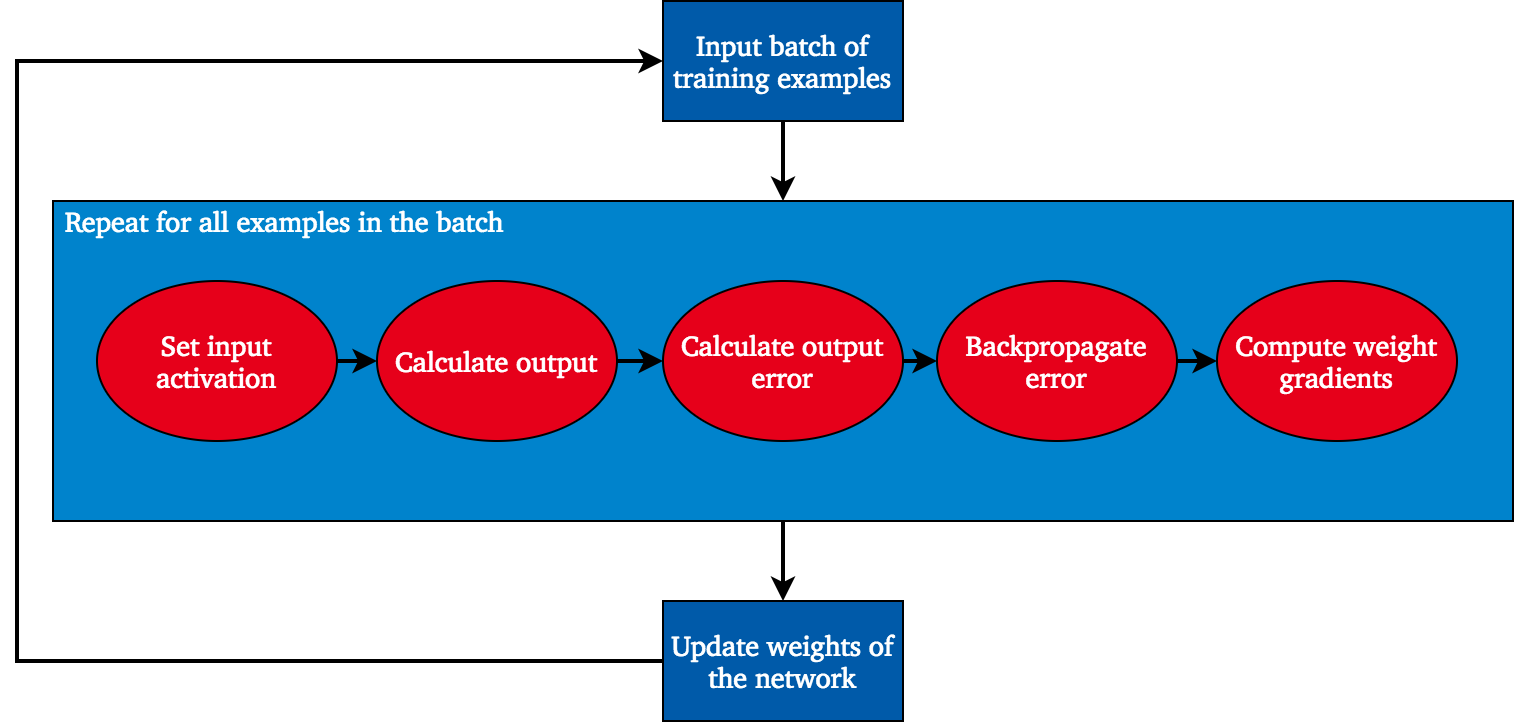
\includegraphics[height=8cm]{img/nn_optimization_3}
  \caption{Optimization in neural networks}
\label{fig:grad_desc}
\end{figure}

All in all, the choice of activation function and optimization algorithm largely
influences efficiency and stability of the learning process.
More sophisticated optimization algorithms will be introduced in the next
subsection, along with recent advances regarding architectures and
regularization techniques.


\subsubsection{Recent Developments}
\label{sub:dl_developments}

After basic paradigms of training neural networks were introduced in the last
subsection, this chapter dives deeper into more sophisticated approaches
which were developed in the last years of deep learning research.
Therefore, the first part explains the drivers behind current progress in the
field (ch.~\ref{sub:dl_drivers}). More complex network architectures which enable
broader practical application will be discussed afterwards (ch.~\ref{sub:dl_architectures}),
before the remaining sections describe modern approaches to optimization
(ch.~\ref{sub:dl_optimization_algos}) and regularization of the training process
(ch.~\ref{sub:dl_regularization}).

\paragraph{Drivers}
\label{sub:dl_drivers}

Progress in deep learning research is mainly enabled by two factors, namely
increased data availability and improved hardware for computation.
Both factors will be detailed in the following.

The term \textbf{big data} is used to describe the phenomenon of increased data
availability.
Main causes for this are migration of transactions from the physical world
to the internet, wide spread of mobile devices like smartphones and success
of social networks, e.g., \textit{Facebook} and \textit{Twitter}.
Big data can best be described by the three dimensions volume, velocity and
variety, also known as the \textit{Three V's}.
Here, \textbf{volume} describes increases in created data, mainly over the 
internet. 
Where volume refers to total size of data sets, \textbf{velocity} stands for the
speed-up in data access. More and more data can be consumed in (nearly) real-time,
e.g., over streaming interfaces.
In addition, big data comes in more diverse form, which is where the \textbf{variety}
dimension has to be regarded.
User-generated images and videos, as well as sensor or GPS data from smartphones
are examples for data types which complement more traditional text and relational
data.
Companies making use of big data in the form of data-driven decision making
have been shown to be more profitable and productive than companies that do not
apply such practices~\footcite{McAfee2012}.
Modern world connectedness makes it possible to store data coming from
many different sources and process it in centralized manner, e.g., to offer
individualized services for consumers~\footcite{Jordan2015}.
Deep learning profits from big data, particularly because models become more
precise with larger data sets.
Large data sets have been shown to improve model performance more than careful
feature engineering, which is required for most machine learning algorithms~\footcite{Goodfellow2016}.
This trend is exemplified in growing benchmark data sets for deep learning
models.
For example, the \textit{MNIST} data set contains 70,000 images of size 28$\times$28 
pixels and served as a benchmark for image recognition since being first
introduced in 1998~\footcite{LeCun1998}.
Nowadays, the most commonly used benchmark for the same task is the \textit{ImageNet}
database, which consists of about 1.2 million images in higher 
resolution~\footcite{Russakovsky2015}.

Processing larger data sets demands a higher number of necessary computations.
Hence, \textbf{computational resources} have to evolve in order to calculate models
in a timely manner.
Deep learning models are most commonly trained using \textit{graphics processing
units} (GPUs), which were formerly applied to highly parallelized processing
in computer games.
GPUs are preferred over CPUs for these tasks, because they contain more
processing units which can carry out computations in parallel.
Graphics processors enable training of more complex models, i.e., models which
contain more neurons and thus learn representation with higher numbers of 
parameters~\footcite{Goodfellow2016, Raina2009}.

\begin{figure}[h]
  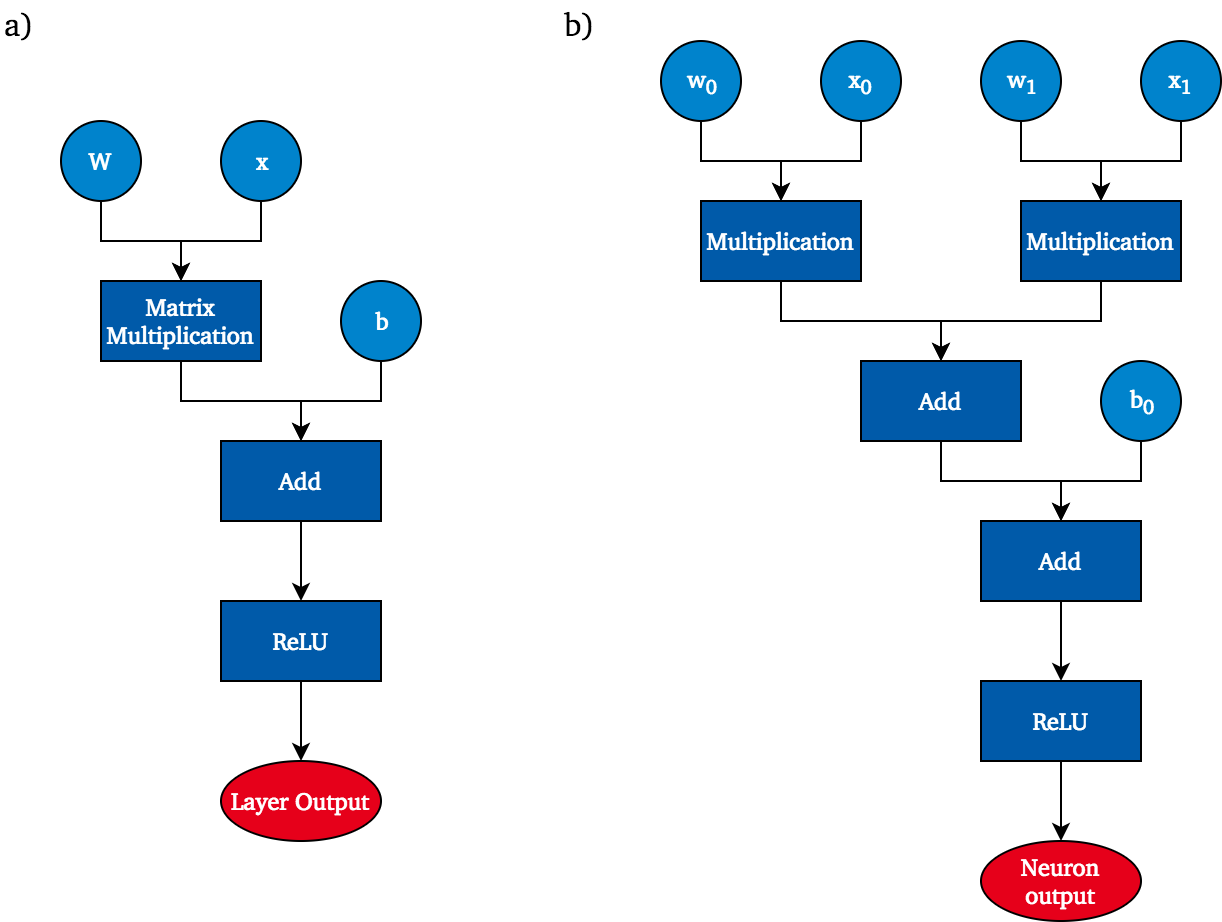
\includegraphics[height=10cm]{img/computation_graph_3}
  \caption[Computation graph for single layer and neuron]{Left: computation graph for a single layer \\ Right: computation graph for a single neuron}
\label{fig:comp_graph}
\end{figure}

Modern deep learning frameworks such as \textit{TensorFlow}\footnote{\url{https://www.tensorflow.org/}}
make use of GPUs by computing neuron outputs for a single layer in parallel.
Forward and backward propagation can be visualized using \textbf{computation
graphs}, which exemplify the single operations for calculating layer outputs.
Figure~\ref{fig:comp_graph}a shows a computation graph for the forward
pass through a fully-connected layer, as introduced in chapter~\ref{sub:dl_forward}.
Instead of computing the matrix operations on a single processing unit, the
calculation can be broken down into less complex subtasks.
Figure~\ref{fig:comp_graph}b exhibits the computation of a single neuron output
from a two-dimensional input vector $x$, which is obviously independent of
other activation computations in the same layer.
Most notably, matrix operations are replaced with element-wise calculations here.
Deep learning software typically computes forward and backward pass in this way
layer by layer in order to speed up the training process~\footcite{Abadi2016}.

This work applies modern deep learning software and hardware for its model.
Exact specifications can be found in chapter~\ref{ch:methodology}.

\paragraph{Network architectures}
\label{sub:dl_architectures}

Above described drivers enable training of more complex models for various
tasks.
In detail, these models contain more parameters and thus possess higher
representational capability.
Over decades of neural network reserach, specialized architectures have been
developed for tasks like image or speech recognition.
This subsection will present three network architectures, two of which will
be used for the model of this work.
For better understanding the architectures are compared to the basic fully-
connected model from chapter~\ref{sub:dl_concepts}

\begin{figure}[h]
  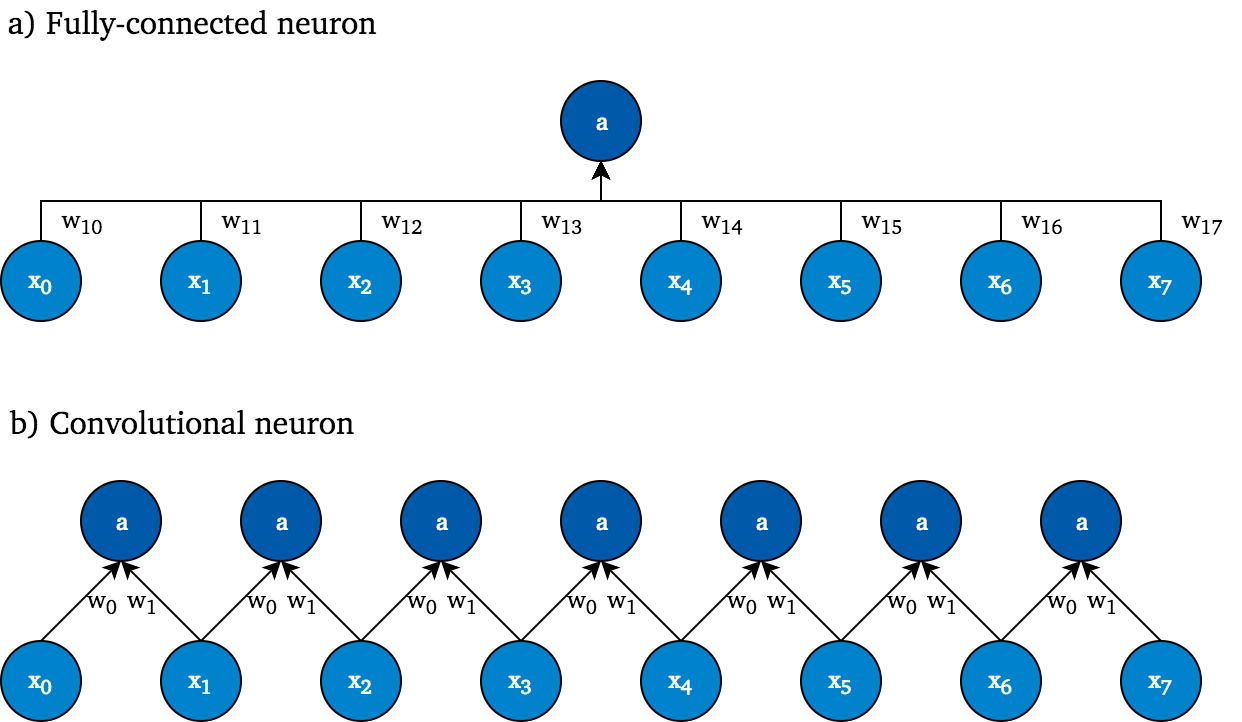
\includegraphics[height=8cm]{img/conv_layer.png}
  \caption{Comparison of fully-connected and convolutional neuron}
\label{fig:conv_layer}
\end{figure}

\textbf{Convolutional neural networks} were first developed by LeCun et al. in 1998,
based on approaches that had been invented during the 1980s~\footcite{Fukushima1980, LeCun1998}.
At that time they were mostly used for simple image processing tasks like
automatic character recognition from handwriting.
In order to understand what characterizes convolutional layers, it is helpful
to compare them to fully-connected layers.
Figure~\ref{fig:conv_layer} compares both layer types for a one-dimensional
input vector and a single neuron in the network layer.
In a fully-connected layer, all inputs are connected to the same neuron.
Contrary, in a convolutional layer, a fixed number of neighboring inputs (two in this example)
are connected to a neuron copy.
All neuron copies share the same weights, as denoted in Fig.~\ref{fig:conv_layer}b,
and thus learn a shared representation of some pattern.
For convolutions to make sense, the ordering of inputs has to be relevant.
This is the case for several data types, e.g., image, text or speech data.
Images will be used as an example here, because the effects of applying
convolutions can be visualized.
Intuitively, one can imagine a convolution as a neuron that is moved over the
vector of inputs and looks for one specific pattern.
For images, a convolution can thus be thought of as a filter that represents
a common reoccuring visual theme.
What kind of pattern (also called \textit{filter}) is learned by the neuron is
determined during the training process.

\begin{figure}[h]
  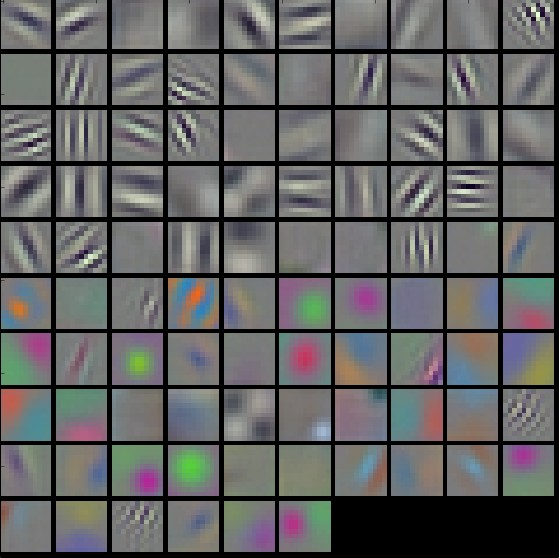
\includegraphics[height=8cm]{img/conv_filters.jpeg}
  \caption[Example filters in a convolutional layer]{Example filters in a convolutional layer~\footcite{Krizhevsky2012}}
\label{fig:conv_examples}
\end{figure}

Figure~\ref{fig:conv_examples} shows examples for such filters, as found in
a large convolutional neural network~\footcite{Krizhevsky2012}.
The top half of filters identify edges of varying orientation and thickness,
whereas the bottom half of filters focuses on color contrasts.
These are examples for filters learned in the first convolutional layer of a
network, that set a new benchmark for image recognition tasks.

\begin{figure}[h]
  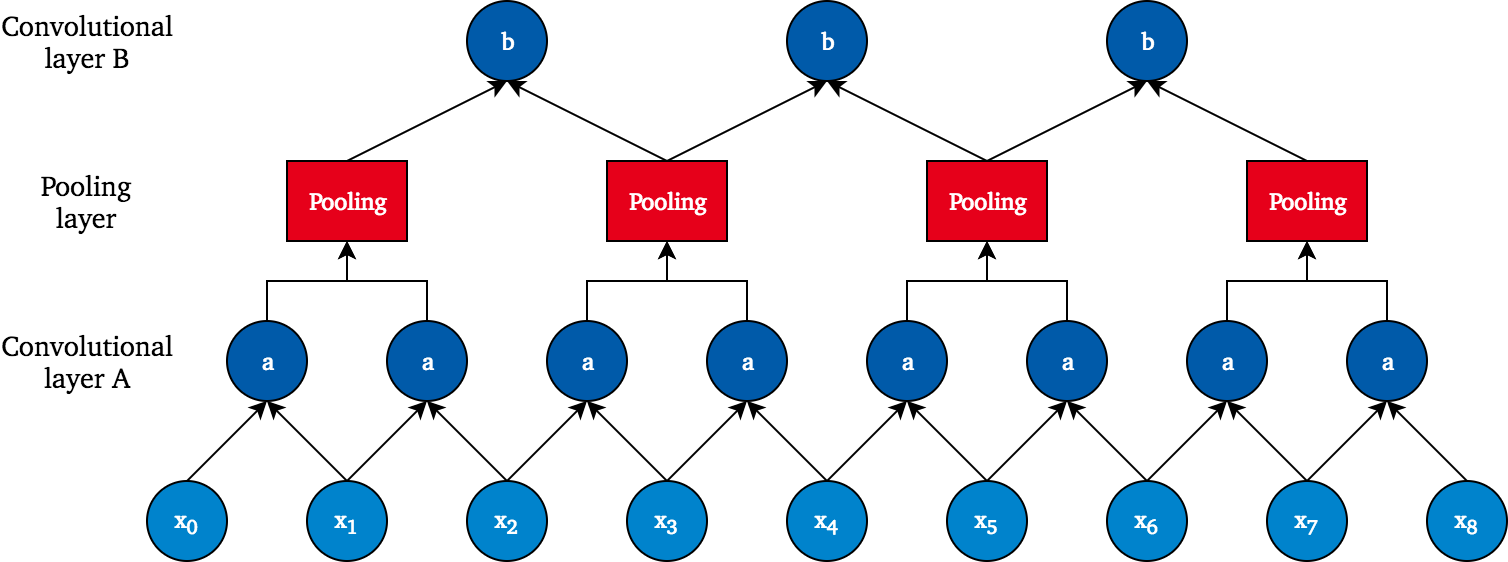
\includegraphics[height=6cm]{img/conv_architecture}
  \caption{Convolutional neural network}
\label{fig:cnn_architecture}
\end{figure}

In practice, convolutional layers are stacked, so that later layers can learn
to identify increasingly complex shapes, e.g., faces or objects, from more
primitive shapes like edges and color contrasts~\footcite{Simonyan2015}.
\textit{Pooling layers} are often used to combine the output of neuron copies, which
enables the next convolutional layer to detect shapes from a greater portion of
the image effectively.
This effect is visualized in Fig.~\ref{fig:cnn_architecture}, where the first
neuron copy of layer $B$ learns a filter from the output of two neuron copies
of layer $A$.
As an example, if layer $A$ learns to detect a horizontal edge, layer $B$ can
find occurrences of two parallel edges in an image.

As mentioned before, convolutional neural networks are mostly applied to data
like images and texts.
More details about practical applications will be discussed in chapter~\ref{sub:dl_applications}.

Like convolutional neural networks, \textbf{recurrent neural networks} (RNNs) are usually
used on data that underlies some kind of ordering.
Popular applications of RNNs lie in the  area of \textbf{Naturual Language
Processing (NLP)}, because text can be formalized as an ordered sequence of
words.

\begin{figure}[h]
  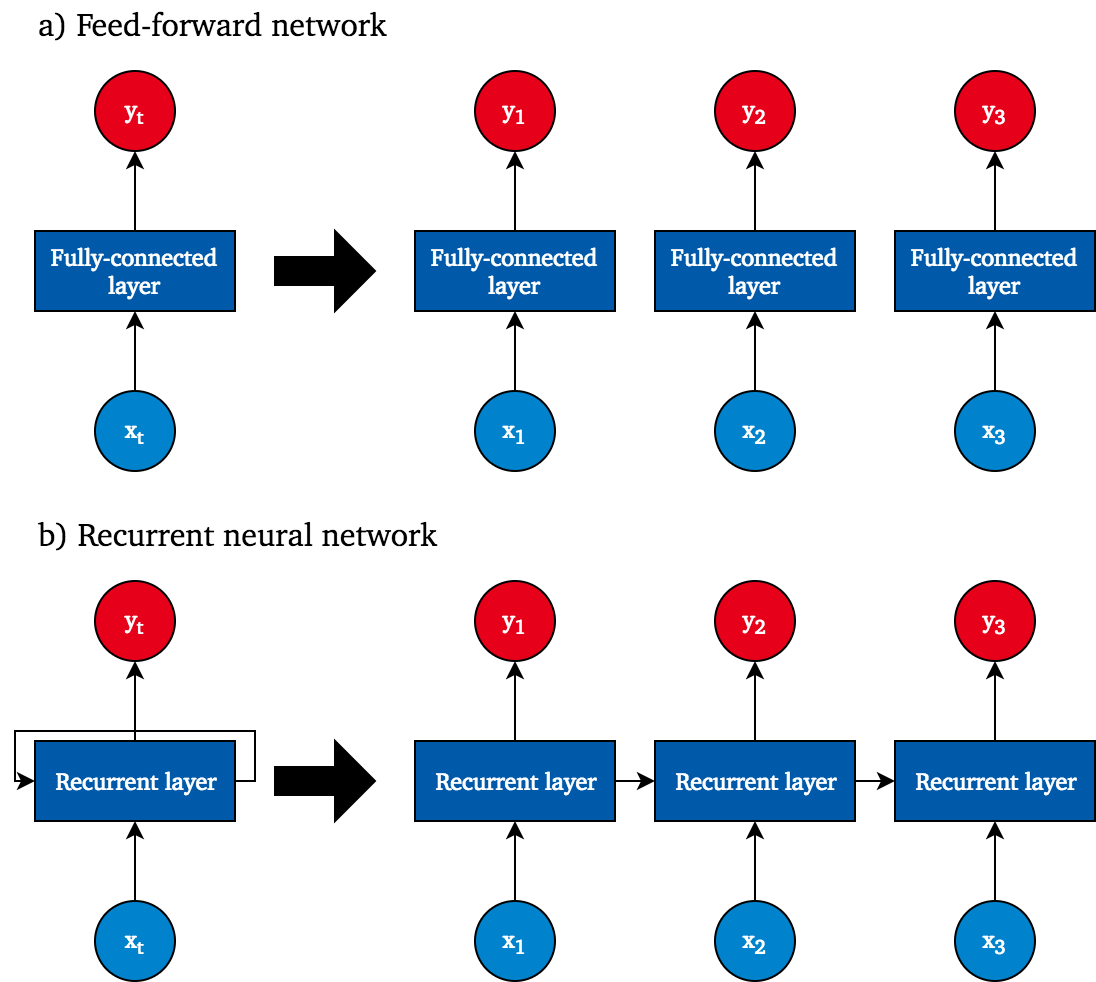
\includegraphics[height=10cm]{img/rnn_unrolled_2}
  \caption{Comparison between unrolled feed-forward and recurrent neural network}
\label{fig:rnn_unrolled}
\end{figure}

One drawback of basic feed-forward networks (see chapter~\ref{sub:dl_concepts})
when looking at ordered sequences is the lack of persistence between single
iterations.
Thus, when looking at an example $x_t$ the network does not know about previous
examples, e.g., $x_{t-1}, x_{t-2},\cdots$.
This fact is exemplified in Fig.~\ref{fig:rnn_unrolled}a, which unrolls a
feed-forward network containing one fully-connected layer into single iterations.
Intuitively, knowing about formerly observed events is useful in many use cases,
e.g., translation tasks or time-series forecasting.
Recurrent neural networks overcome the liability by introducing the concept
of \textbf{memory}.
As shown in Fig.~\ref{fig:rnn_unrolled}b, information is passed between
iterations, which for example enables the network to memorize previous inputs~\footcite{Goodfellow2016}.
The most applied RNN variant is the so-called \textbf{Long Short-Term Memory}
network, which will be explained in the following.

\begin{figure}[h]
  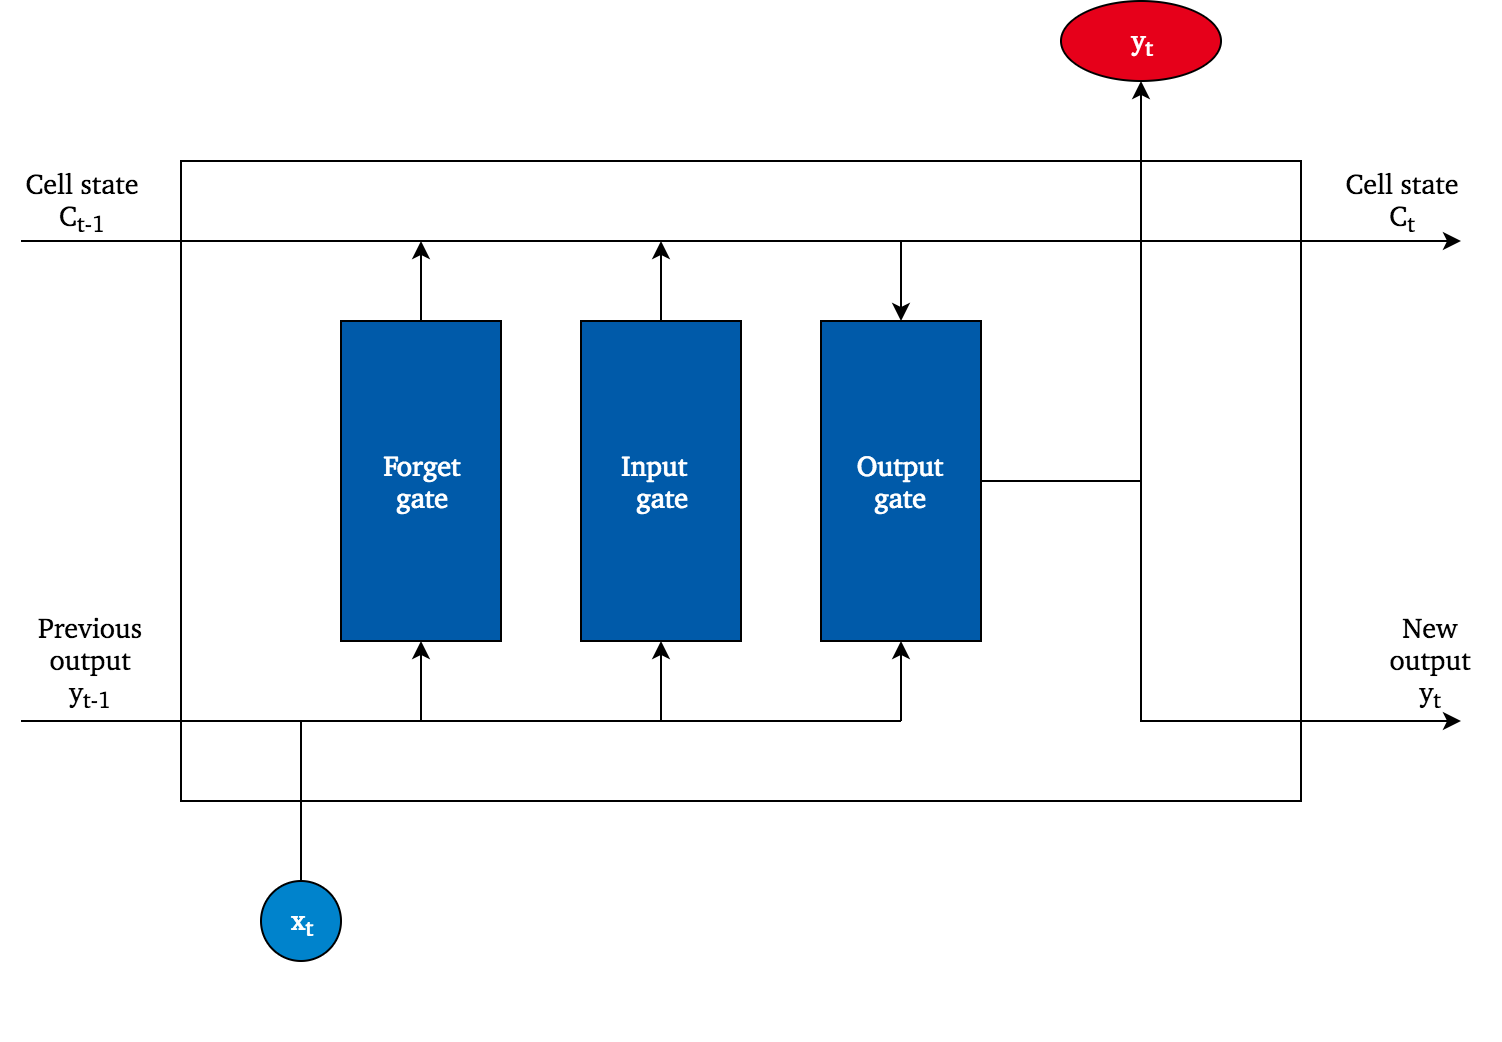
\includegraphics[height=11cm]{img/lstm_cell}
  \caption{Simplified LSTM cell}
\label{fig:lstm_cell}
\end{figure}

The Long Short-Term Memory (LSTM) network was first introduced by Hochreiter \&
Schmidhuber~\footcite{Hochreiter1997} in 1997, aiming to solve the problem of
storing information in a neural network over time.
A LSTM neuron (often calledLSTM cell) comprises four separate layers which 
manipulate the \textit{cell state}.
The cell state stores information and is passed between iterations of the
training process.
In summary, the four included layers serve three purposes: removing unnecessary
information, adding new information and creating an output.
The three tasks are handled in \textit{gates} which contain the necessary
network layers for computation and are responsible for editing the cell state
accordingly.
The following explanations of LSTM gates are illustrated in Fig.~\ref{fig:lstm_cell}.

All three gates process the current input $x_t$ and the output of the previous
iteration $y_{t-1}$.
LSTMs are commonly applied for Natural Language Processing tasks such as
language modeling, i.e., prediction of the next word based on previously seen
text.
Therefore, an example language modeling task will be used to describe the
gate functionalities~\footcite{Olah2015}.
Firstly, the \textit{forget gate} decides which information can be removed from
the cell state.
Internally, the forget gate contains a simple layer with sigmoid activations.
Outputs of the layer are multiplied element-wise with the cell state.
The activations are guaranteed to be between zero and one, where zero represents
`forgetting' and one stands for `keeping' information.
For example, when trying to predict words in a sequence it is necessary
to know about the current subject in order to conjugate an upcoming predicate
correctly.
If the current input $x_t$ represents a new subject, e.g., `he',the old subject should
probably be removed from the cell state in the forget gate.
Secondly, the \textit{input gate} is responsible for adding new information to the cell
state.
It does so in two distinct steps, which are processed in separate layers.
Here, the first decision is which information to update, and the second one
which new values to add.
The layer outputs are combined using the Hadamard Product and then added to the
cell state.
Continuing previous example, the input gate would likely add information about
the gender of the new subject, which determines word endings for predicates in
many languages.
Finally, an output for the current iteration is generated in the \textit{output gate}.
The output represents `a filtered version'~\footcite{Olah2015} of the cell state, e.g.,
information for upcoming verbs when a new subject is observed.
This happens through the use of another layer with sigmoid activations which
intuitively filters relevant information from the cell state.
As can be seen in Fig.~\ref{fig:lstm_cell}, the output is also passed to the
next iteration.

LSTMs have been applied to problems ranging from speech recognition to
image captioning, which require storing input information with regard to the
training process.
Architectures using multiple, stacked LSTM layers are also used in practice,
mainly to learn even more complex representations.
Detailed use cases will be a central theme in Ch.~\ref{sub:dl_applications}.

The previously described architectures of CNNs and RNNs were developed prior to
the third wave of neural network research and became efficiently trainable
due to driving factors described in Chapter~\ref{sub:dl_drivers}.
Finally, this subsection introduces \textbf{Generative Adverserial Networks (GANs)}, which
represent a more recently invented model architecture.
The basic concept was presented by researchers in 2014, and has gained popularity
since then~\footcite{Goodfellow2014}.
As can be extracted from the name, GANs belong to the family of \textit{generative
models}.
In contrast to \textit{discriminative models} which learn a decision boundary
between classes (e.g., Support Vector Machines), generative models implicitly 
model the probability distribution of inputs and outputs~\footcite{Bishop2006}.
Therefore, generative models can be used to generate new data from the learned
distribution, e.g., new images can be created from a sample of real images.
Generative adversarial networks approach this problem by combining two neural 
networks into a single model, as illustrated in Fig.~\ref{fig:gan_architecture}.

\begin{figure}[h]
  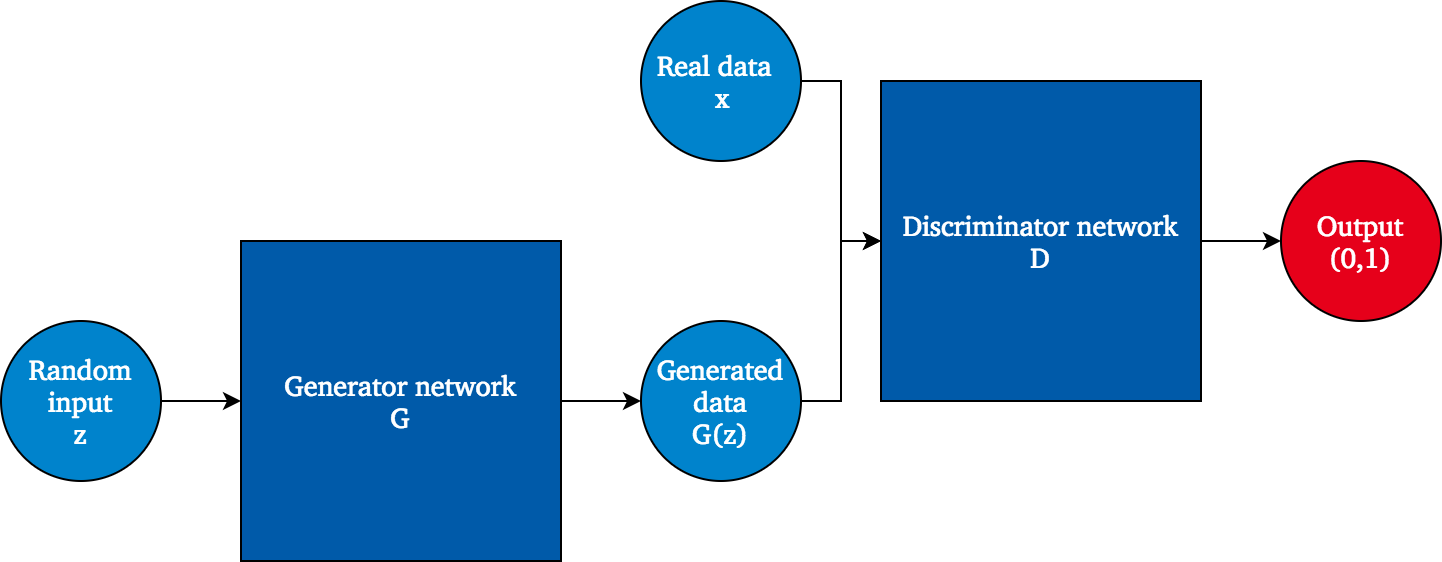
\includegraphics[height=6.5cm]{img/gan_architecture}
  \caption{Architecture of a Generative Adversarial Network (GAN)}
\label{fig:gan_architecture}
\end{figure}

In general, a GAN consists of a \textit{generator network G} and a \textit{discriminator network D}.
The generator outputs new data $G(z)$ from a random input vector $z$ which is
drawn from a normal distribution.
The generated data then serves as an input to the discriminator, along with
real data $x$.
Tasked with distinguishing between real and generated data, the discriminator
outputs probabilities representing an estimation of the authenticity of an
example.
Intuitively, the aim of the GAN architecture is to create new samples that carry
such similarity with original samples, that the discriminator can not differentiate
between real and generated anymore.
The question arises, how this objective can be expressed in a cost function.
Traditionally, generative models were trained by minimizing the distance of
generated output to nearest sample in the real data~\footcite{Goodfellow2014}.
GANs use a different objective function, which is exemplified in equation~\ref{eq:gan_obj}.

\begin{equation}
  \label{eq:gan_obj}
  \min_G \max_D V(D, G) = \mathbb{E}_{x \sim p_{data}(x)}[\log D(x)] + \mathbb{E}_{z \sim p_z (z)}[\log (1 - D(G(z)))]
\end{equation}

The cost function includes the objectives of both networks, as the generator
tries to minimize the above equation and the discriminator aims to maximize it.
Both terms represent in the equation represent log-likelihood functions.
Maximizing the equation means assigning the correct labels to data samples (aim
of the discriminator), minimizing it implies that the discriminator is not capable
of specifying where a sample comes from (aim of the generator).
The authors of the original paper prove the existence of a unique solution, where
the generator is able to represent the original data distribution and the 
discriminator outputs probabilities of 0.5 for every sample~\footcite{Goodfellow2014}.
Such a game between two entities following conflictive objectives is referred to
as a \textit{minimax setting}~\footcite{Russell1995}.

During the training process, weights for both networks have to be updated.
This can be achieved through backpropagating errors through both networks,
although some adaptations have to be made.
Training processes as follows:

\begin{enumerate}
  \item Determine architecture for generator and discriminator network
  \item Update $D$ while $G$ is not trainable and samples are split between real and generated
  \item Update $G$ while $D$ is not trainable and samples are all generated
  \item Repeat steps 2 and 3 for desired number of iterations
\end{enumerate}

It becomes obvious that the two networks are updated alternatively.
An important caveat is that one network is not trainable, i.e., the weights are
fixed, while the other one is updated.
Fixed weights are not updated during training, but solely used to pass information
forward and backward through the network.

GANs were applied to creation of images in the original paper, but have been
used for a bigger variety of problems since. As for the other architectures,
more practical applications can be found in Ch.~\ref{sub:dl_applications}.
After examining more advanced architectures, the next two subsections will
focus on the training process.
In particular, developments in optimization algorithms and regularization
techniques are described.

\paragraph{Optimization algorithms}
\label{sub:dl_optimization_algos}

The choice of optimization algorithms influences the stability of the training
process.
Here, the aim is to converge to a good solution in reasonable time, ideally
finding a minimum for the cost function by adapting weights in the network.
Chapter~\ref{sub:backprop} introduced a basic structure for optimization
algorithms in neural network training, as well as update functions for the
\textit{stochastic gradient descent} optimization algorithm.
Basically, gradient descent only relies on derived gradients and a hyperparameter
representing the learning rate, i.e., the step size towards a possible minimum
(~\ref{eq:gd}).
For complex neural networks, gradient descent can be hard to utilize effectively.
Suitable, often manual weight initialization and adaptions of the learning rate
during training are needed in order to derive good solutions.
More sophisticated optimization algorithms, which were developed in the last
years, overcome these limitations.
This subsection will first introduce the concept of \textit{momentum} in
numerical optimization and then explain a commonly deployed algorithm called
\textit{Adam}.

\begin{equation}
  \label{eq:gd}
  w_{t+1} \rightarrow w_t - \eta \nabla f(w_t)
\end{equation}

The concept of \textbf{momentum} was developed in the 1960s and has since been applied
to numerical optimization problems~\footcite{Polyak1964}.
During the third wave of neural network research, the concept was first
utilized for accelerating training processes in deep networks~\footcite{Sutskever2013}.
In its essence, momentum (equation~\ref{eq:momentum}) adds an additional step to 
the gradient descent update function (equation~\ref{eq:gd}).

\begin{align}
  \label{eq:momentum}
  v_{t+1} \rightarrow \mu v_t + \eta \nabla f(w_t) \\
  w_{t+1} \rightarrow w_t - v_{t+1}
\end{align}

The weight update $v_{t+1}$ is composed by two terms: the gradient $\nabla f(w_t)$
weighted with the learning rate $\eta$ and the previous update $v_t$ multiplied
with the \textit{momentum coefficient} $\mu$.
Therefore, the update in iteration $t+1$ depends on the update of iteration $t$,
which again is dependent on $v_{t-1}$ and so on.
The added term $\mu v_t$ can thus be interpreted as an exponentially moving 
average of previous updates, where hyperparameter $\mu$ determines the magnitude 
of influence of these predecessor updates.
Momentum allows the optimizer to progress more evenly without too many changes
of direction.
This overcomes the liability of gradient descent which is susceptible to
frequent changes of directions in the gradient, e.g., if examples in a mini-batch
are particularly noisy.

As outlined in above paragraph, momentum keeps track of the exponentially moving
average of previous gradients.
This added average constitutes a first moment estimate of the gradients, also 
known as \textit{mean estimate}.
The \textbf{adaptive moment estimation (Adam)} optimization algorithm enhances
momentum with further computations in order to guarantee accelerated
convergence~\footcite{Kingma2014a}.
Intuitively, Adam adapts the learning rate for each parameter based on mean and
variance of recent updates in the specific parameter.
Equations~\ref{eq:adam_start} through~\ref{eq:adam_end} exemplify the update
computation for a single parameter $w$ in iteration $t$.

\begin{align}
  g_t &= \nabla f(w_t) \label{eq:adam_start} \\
  m_t &= \beta_1 m_{t-1} + (1-\beta_1) g_t \label{eq:adam_2} \\
  v_t &= \beta_2 v_{t-1} + (1-\beta_2) g_t^2 \label{eq:adam_3} \\
  \widehat{m}_t &= \frac{m_t}{1-\beta_1^t} \label{eq:adam_4} \\
  \widehat{v}_t &= \frac{v_t}{1-\beta_2^t} \label{eq:adam_5} \\
  w_{t+1} &= w_t - \frac{\eta}{\sqrt{\widehat{v}_t} + \epsilon} \widehat{m}_t \label{eq:adam_end}
\end{align}

Equations~\ref{eq:adam_2} and~\ref{eq:adam_3} compute mean and
uncentered variance estimates of the gradient, similar to momentum.
$\beta_1$ and $\beta_2$ are hyperparameters, whose default values are $0.9$ and
$0.999$ respectively.
Because of these defaults and zero initialization of $m$ and $v$, the estimates
are biases towards zero, especially in early iterations.
This bias is corrected in equations~\ref{eq:adam_4} and~\ref{eq:adam_5}, where
the scaling factor $\frac{1}{1-\beta_1^t}$ is larger for smaller values of $t$
and therefore accounts for smaller values of the estimates as a result of 
zero initialization.
Final updates are then calculated via the corrected estimates and hyperparameters
$\eta$ (representing the learning rate) and $\epsilon$ (defaults to $10^{-8}$).

\begin{figure}[h]
  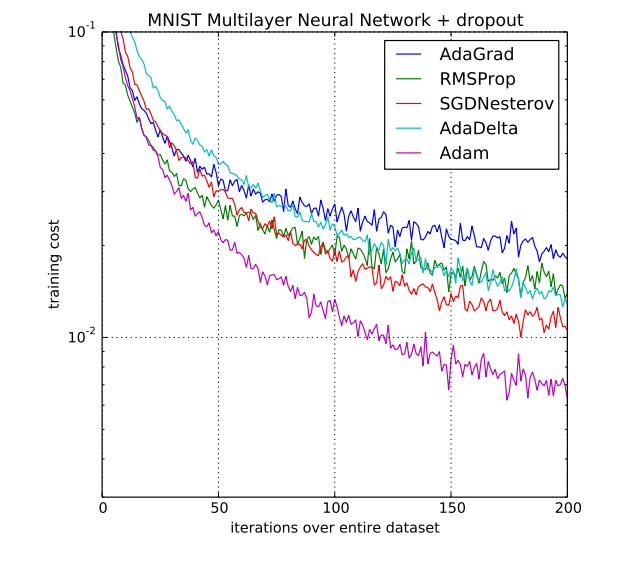
\includegraphics[height=10cm]{img/adam_comparison}
  \caption[Comparison of optimization algorithms]{Comparison of optimization algorithms~\footcite{Kingma2014a}}
\label{fig:adam_comp}
\end{figure}

Kingma \& Ba~\footcite{Kingma2014a} list concise implementation, computational efficiency,
suitability for complex models with many parameters and reasonable default values
for the hyperparameters as main benefits of adaptive moment estimation.
Figure~\ref{fig:adam_comp} compares Adam to other optimization algorithms,
applied in the context of a deep neural network with the task of handwriting
recognition.
It can be seen that Adam achieves a better solution, i.e., lower value of the
cost function, over the course of 200 iterations.

\paragraph{Regularization techniques}
\label{sub:dl_regularization}

In addition to optimization algorithms, regularization techniques largely
influence training process stability and generalization ability of the
resulting model.
These techniques are particularly helpful for complex models such as deep
neural networks, and custom methods have been developed during the current
research wave.
This subsection will introduce regularization procedures after firstly explaining
the concept of overfitting which many techniques aim to prevent.

\textit{Generalization} constitutes the main challenge in machine learning and
denotes the ability to `perform will on new, previously unseen inputs'~\footcite[110]{Goodfellow2016}.
Therefore, machine learning models should not only be evaluated using training
error, i.e., the performance measure on training data, but also via \textit{test
error}, i.e., the performance on unseen test data.
In summary, key objectives of machine learning algorithms can be put as follows:

\begin{enumerate}
  \item Minimize training error
  \item Minimize gap between training and test error
\end{enumerate}

\begin{figure}[h]
  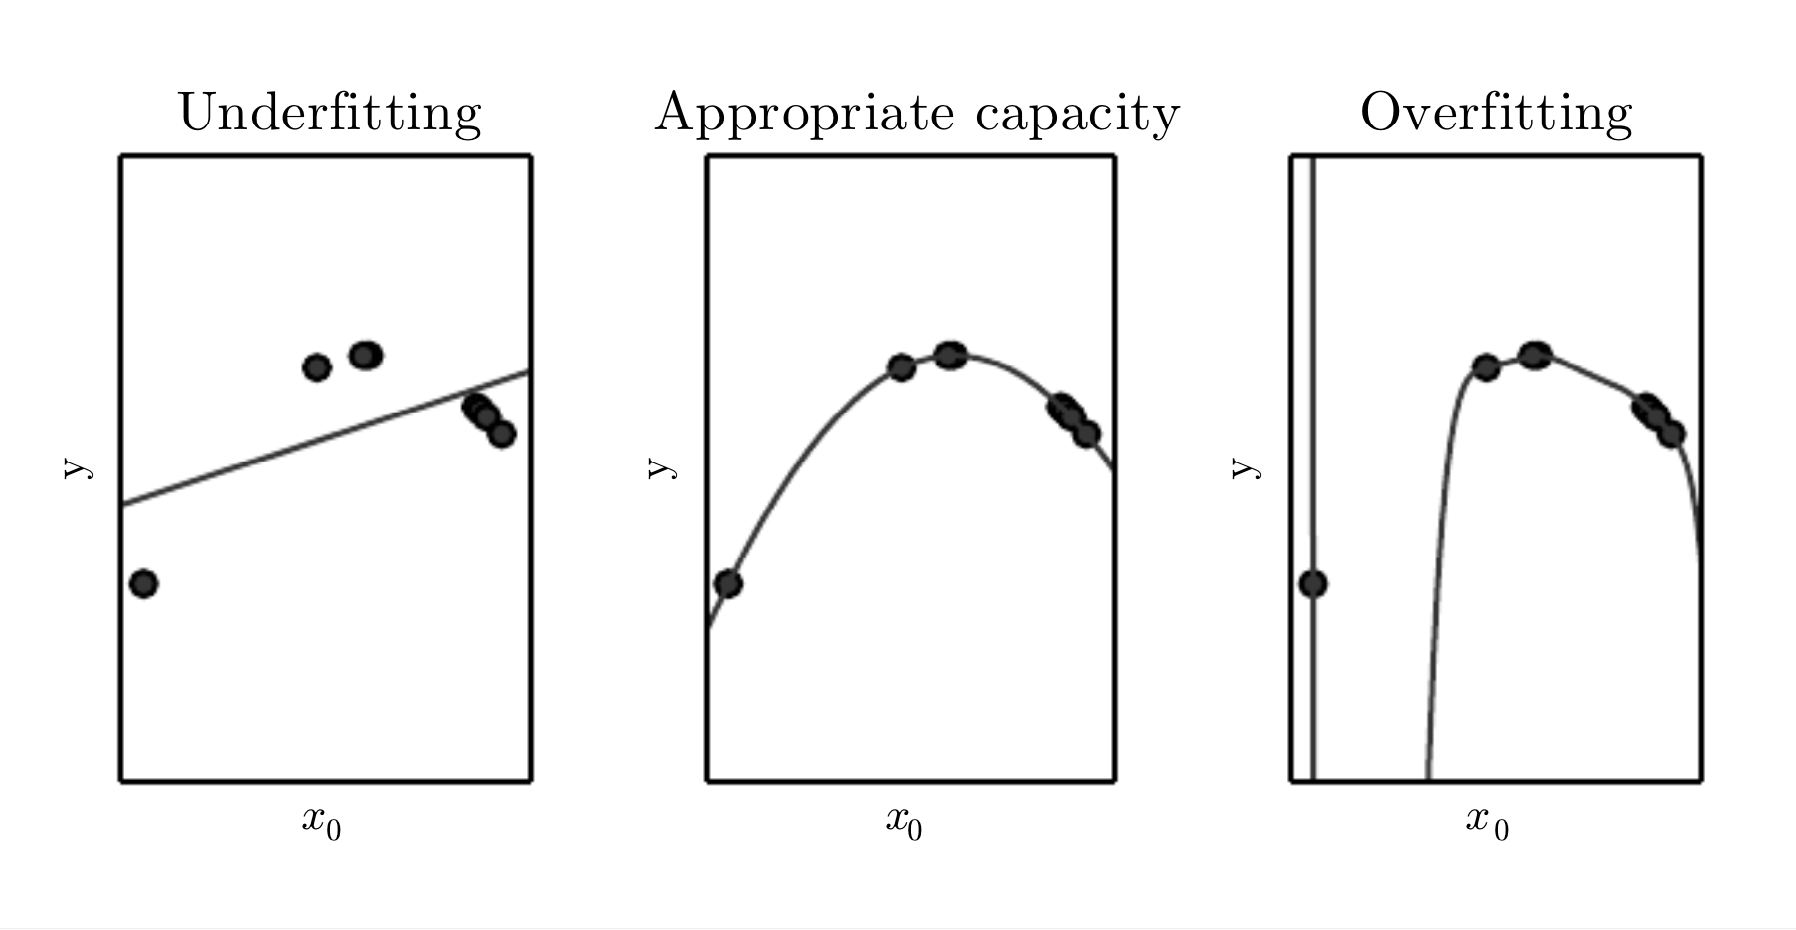
\includegraphics[height=8cm]{img/overfitting}
  \caption[Overfitting, underfitting and appropriate capacity]{Overfitting, underfitting and appropriate capacity~\footcite{Goodfellow2016}}
\label{fig:overfitting}
\end{figure}

\textbf{Overfitting} simply refers to a large gap between training error and test
error.
Intuitively, the model learns too much about specific examples in the training
set and can not perform well on other data.
In contrast to that, \textit{underfitting} occurs when the model is not able
to explain a significant portion of variance in the data.
Fig.~\ref{fig:overfitting} displays examples for both phenomena, as well as
an appropriate model in the context of curve fitting.
Overfitting is often a result of long-running training processes which are
not regularized appropriately.
The following paragraphs describe techniques commonly used to avoid overfitting.

\textbf{Dropout} aims to solve a commonly occurring problem in deep neural networks
called `co-adaption'~\footcite{Hinton2012a}.
It refers to neurons that detect features whose usefulness can not be isolated,
but is dependent on the detection of other features.
Such a neuron is only helpful in conjunction with other neuron.
Co-adaptation can cause overfitting, because it creates an opportunity for
the network to model patterns in the training data in an excessively detailed
way.
Contrary, neurons should learn to detect features that are useful in isolation.
Applying dropout refers to random deactivation of a prespecified percentage
of neurons.
Neurons that are omitted in this way, are removed on the forward pass of an
iteration.
This can be achieved by setting the activations to zero instead of computing
them.
On the backward pass, weights that are connected to deactivated neurons receive
no updates.
The only necessary parameters for each layer using droput is the percentage
of active neurons $p$.
This represents the probability that the neuron is present during training.
When applying the network to test data, all units are present to make predictions.
However, weights from all network layers using dropout are multiplied by $p$.
This makes the application of dropout straighforward.
Despite its algorithmic simplicity, dropout has been shown to reduce overfitting
in several deep architectures~\footcite{Srivastava2014}.

Another, even more recently developed regularization technique is \textbf{batch
normalization}.
It addresses the problem of slowly converging training processes caused by
\textit{internal covariate shift}, which is the amount by which layer activations
change over the course of many iterations.
This amount is influenced by the fact that the distribution of layer activations changes
as the parameters connected to it are updated.
In order to deal with varying activation distributions the learning rate often
has to be lowered which in turn can slow down network training considerably.
Batch normalization addresses this problem by normalizing layer inputs for
a mini-batch of examples in an iteration.
Intuitively, this makes sense since data is often normalized in preprocessing
before being put into a model.
Technically, inputs are normalized along all dimensions $k$ by subtracting the mean
and dividing by the standard deviation of respective dimension (see equation~\ref{eq:bn_norm}).

\begin{align}
  \widehat{x}^{(k)} = \frac{x^{(k)} - E[x^{(k)}]}{\sqrt{Var[x^{(k)}]}} \label{eq:bn_norm} \\
  y^{(k)} = \gamma^{(k)} \widehat{x}^{(k)} + \beta^{(k)} \label{eq:bn_scale_shift}.
\end{align}

Normalizing layer inputs in this way limits internal covariate shift, but also
limits the representational capability of these neurons.
Therefore, batch normalization adds learnable parameters $\gamma$ and $\beta$ for
each input, which serve to scale and shift the input after normalization~\ref{eq:bn_scale_shift}.
Hence, the network can learn to undo the normalization (\textit{denormalization})
if necessary.
Batch normalization has been shown to speed up the training process and also
reduce overfitting which limits the necessity for dropout~\footcite{Ioffe2015}.

\begin{figure}[h]
  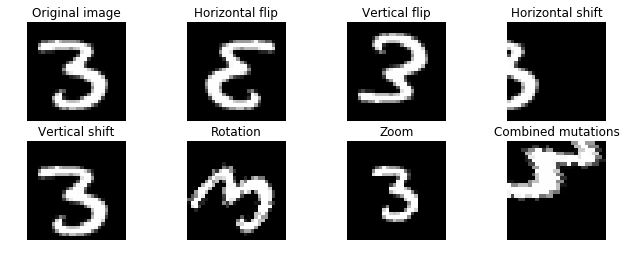
\includegraphics[height=6.5cm]{img/data_augmentation}
  \caption{Self-created examples of augmented images}
\label{fig:augmented_images}
\end{figure}

As described in Chapter~\ref{sub:dl_drivers}, deep neural networks profit from
large amounts of data.
Therefore, the first step in reducing overfitting is usually to add
more data.
This can be achieved using either more real data, or by generating new examples
from already used training data.
This technique called \textbf{data augmentation} is common in computer vision
problems that deal with images~\footcite{Simard2003}.
It refers to the enhancement of training data with variations of existing training
examples.
For images these augmented images can created using minor mutations, e.g., random rotations, flips, shifts or
color changes.
Fig.~\ref{fig:augmented_images} shows examples of a handwritten character being
mutated in various ways.
Data augmentation leads to a bigger variety of inputs, which has been shown
to reduce overfitting for deep neural networks~\footcite{Krizhevsky2012}.


\subsubsection{Practical Applications}
\label{sub:dl_applications}

The previous chapter section covered recent progress in neural network research
on a theoretical level.
After gaining an understanding of modern architectures and training techniques,
this chapter will present practical applications of deep learning.
The upcoming subsections explain problems from multiple areas of computer
science, that can be approached using neural networks.
Namely, sections cover applications in Natural Language Processing (ch.~\ref{sub:dl_app_nlp}),
Computer Vision (ch.~\ref{sub:dl_app_cv}) and Reinforcement Learning (ch.~\ref{sub:dl_app_rl}).

\paragraph{Natural language processing (NLP)}
\label{sub:dl_app_nlp}

Section~\ref{sub:dl_architectures} introduced the problem of \textit{language modeling},
i.e., learning a probability distribution for words in a given sequence.
Convolutional and recurrent neural networks have been successfully applied to
this problem, in many cases improving previous state-of-the-art performance
on benchmark data sets.
Both network architectures are combined within complex models, so that these
so-called \textit{neural language models} are able to encode multiple
languages~\footcite{Kim2015}.
Another application of neural networks lies in the area of \textit{text classification},
i.e., assignment of a given text or document into predefined categories.
An example for this problem is classification of news articles into classes such
as sports, finance or politics.
This is an additional area in which deep learning shows increased performance
over previous approaches, mostly through the use of deep convolutional neural
networks~\footcite{Conneau2016}.
The most recently solved problem in natural language processing is \textit{machine
translation}, which aims to automate conversion of text between different
languages.
Complexity is here derived from the necessity of encoding the source language and
then decoding the learned representation into the target language.
Both model components, i.e., encoder and decoder, have shown to be efficiently
learnable with LSTMs (see ch.~\ref{sub:dl_architectures})~\footcite{Sutskever2014}.
The practical relevance of this research area is exemplified by contributions
from corporate research departments, e.g., \textit{Google}~\footcite{Wu2016}.

\paragraph{Computer vision}
\label{sub:dl_app_cv}

\begin{figure}[h]
  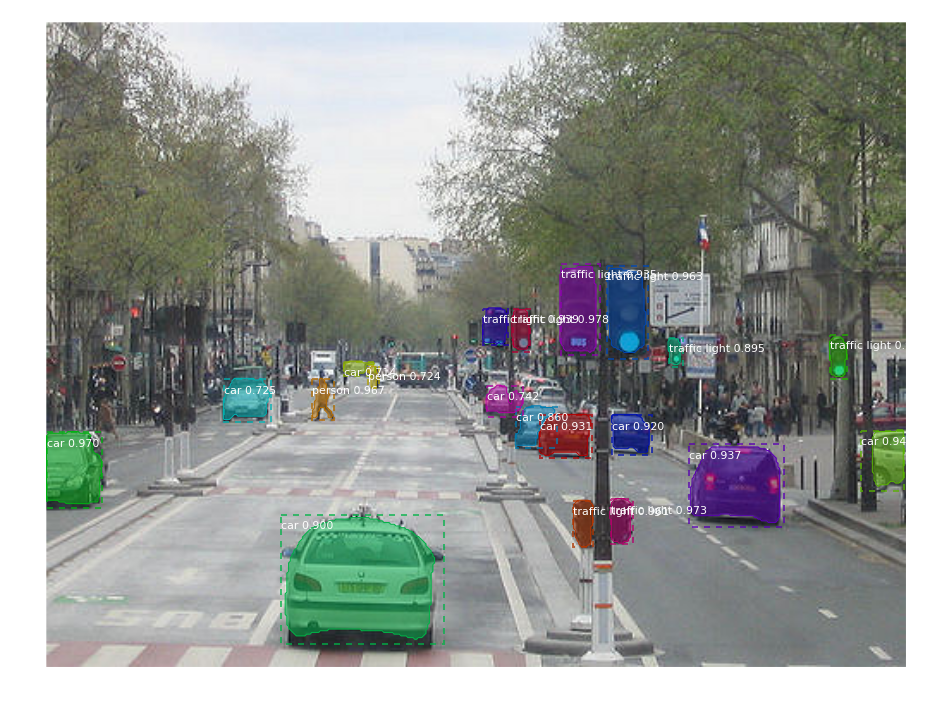
\includegraphics[height=10cm]{img/mask_rcnn}
  \caption[Object detection example]{Object detection example in street scenery~\footnote{\url{https://github.com/matterport/Mask_RCNN}}}
\label{fig:obj_detection}
\end{figure}

The area of computer vision mainly aims to process image and video data in
various ways.
Example problems that are solved using deep learning methods are presented in
the following.
As mentioned in previous chapters, \textit{image recognition} describes the
process of assigning images to categories.
Convolutional neural networks were designed to tackle problems like image
recognition by looking at individual sections of images using filters to
detect common features~\footcite{LeCun1998}.
Progress in deep learning allows training deeper models that contain more
convolutional layers and therefore can learn more complex features.
Thus, deep convolutional networks were able to push the state-of-the-art in image recognition~\footcite{Krizhevsky2012, He2016}.
\textit{Object detection} constitutes a related problem, whose goal is
to find all occasions of a predefined set of objects in an image.
Fig.~\ref{fig:obj_detection} shows an example image from a street scenery
with identified objects such as cars or traffic signals.
Deep learning models applied to object detection usually contain convolutional
layers to identify regions of interest in an image and map these to the
specified object classes~\footcite{Girshick2012, He2017}.
High-performance object detectors can then be used for even more advanced
tasks such as \textit{visual tracking}, i.e., following objects over several video
frames, or \textit{image captioning} which aims to describe images~\footcite{Bertinetto2016, Karpathy2017}.

\begin{figure}[h]
  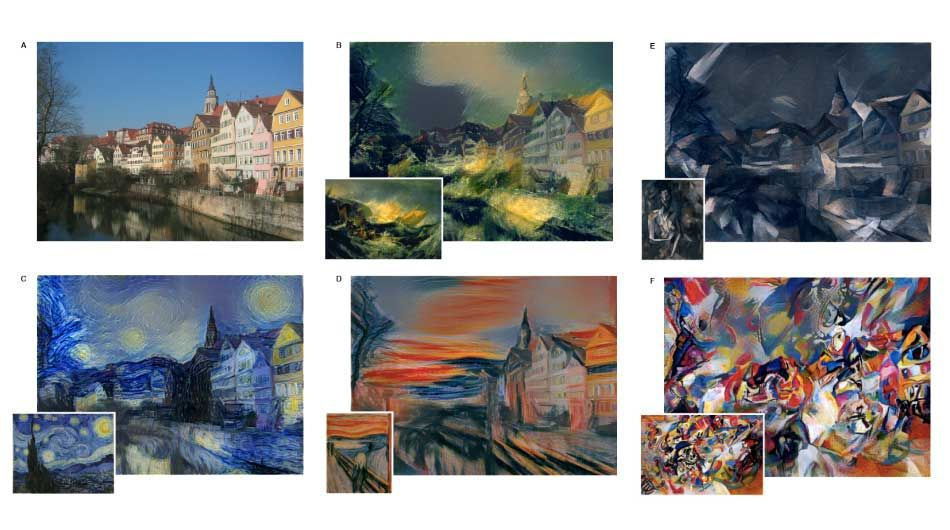
\includegraphics[height=9cm]{img/style_transfer.jpg}
  \caption[Style transfer example]{Style transfer example~\footcite{Gatys2015}}
\label{fig:style_transfer}
\end{figure}

Convolutional neural networks have also been used for generative tasks like
\textit{style transfer}.
Here, the goal is to apply styles of a source image, e.g., texture or colors,
to a target image.
An example is shown in Fig.~\ref{fig:style_transfer}, where a house scenery is
repainted in the style of various artists~\footcite{Gatys2015}.
Related tasks include image generation, where generative adversarial networks
show good performance~\footcite{Radford2015}.
Style transfer and image generation are also examples for unsupervised learning
problems, as introduced in ch.~\ref{sub:dl_terminology}, because there is
generally no labeled data for these tasks.

\paragraph{Reinforcement learning}
\label{sub:dl_app_rl}

Reinforcement learning constitutes another kind of experience for machine
learning algorithms.
In this setting, an agent continuously interacts with its environment and learns
from feedback in the form of rewards.
In order to estimate rewards for specific actions, the current state of the
given setting has to be evaluated.
Deep learning models have mostly been applied to evaluate settings that can
be displayed visually.
For example, this is the case for video games where each video frame represents an image.
Convolutional neural networks are used to detect patterns in the current
setting which are helpful for an agent and its decision about upcoming
actions.
Recently, researchers were able to train agents that perform better than human
professionals in several games, including simple \textit{Atari} video games
and more complex games like \textit{Go}~\footcite{Mnih2015, Silver2016}.

This chapter concludes the covered deep learning theory for this thesis.
The upcoming chapter explains basic concepts of social networks in general and
\textit{Twitter} more specifically, which are necessary for understanding
upcoming experiments.


\subsection{Social Networks}
\label{sec:social_networks}

Applying deep learning to tweet engagement prediction requires a basic
understanding of social network dynamics and structure. Furthermore, a common
understanding of Twitter terminology is necessary for later chapters of this
work. Both areas will be covered in this section, beginning with social
networks in general (ch.~\ref{sub:sn_terminology}) and concluding with
Twitter in detail (ch.~\ref{sub:sn_twitter}).

\subsubsection{Terminology}
\label{sub:sn_terminology}

As with deep learning, social network terminology is sometimes used in confusing
ways.
This subsection aims to eliminate terminology confusion and introduce basic concepts regarding social networks,
as well as related notions like social media.
Firstly, the term \textit{social network} is defined (ch.~\ref{sub:sn_social_networks}), before structural
properties are explained (ch.~\ref{sub:sn_structure} and~\ref{sub:sn_properties}).
The last paragraph of this section focuses on \textit{social media}, especially
practical implications for organizations (ch.~\ref{sub:sn_social_media}).

\paragraph{Social networks}
\label{sub:sn_social_networks}

In order to examine social network structure and properties, the term first
has to be defined.
Wassermann \& Faust (1994) explicate that ``a social network consists of a finite
set or sets of actors and the relation or relations defined on them''~\footcite[20]{Wasserman1994}.
Here, an \textit{actor} can be any social entity, e.g, people, groups, countries or
organizations.
\textit{Relations} are then batches of ties between these entities, e.g., resource
transfers, associations or interactions~\footcite{Wasserman1994}.
With this basic definition set, the next two paragraphs focus on structure and
properties of social networks.

\paragraph{Structure}
\label{sub:sn_structure}

Social networks can be visualized using graphs, where actors serve as nodes
and lines represent relations between these actors.
Thus, the network consists of a set of nodes $N = \{n_1, n_2, \cdots, n_g\}$ and
a set of lines $L = \{l_1, l_2, \cdots, l_L\}$~\footcite{Wasserman1994}.

\begin{figure}[h]
  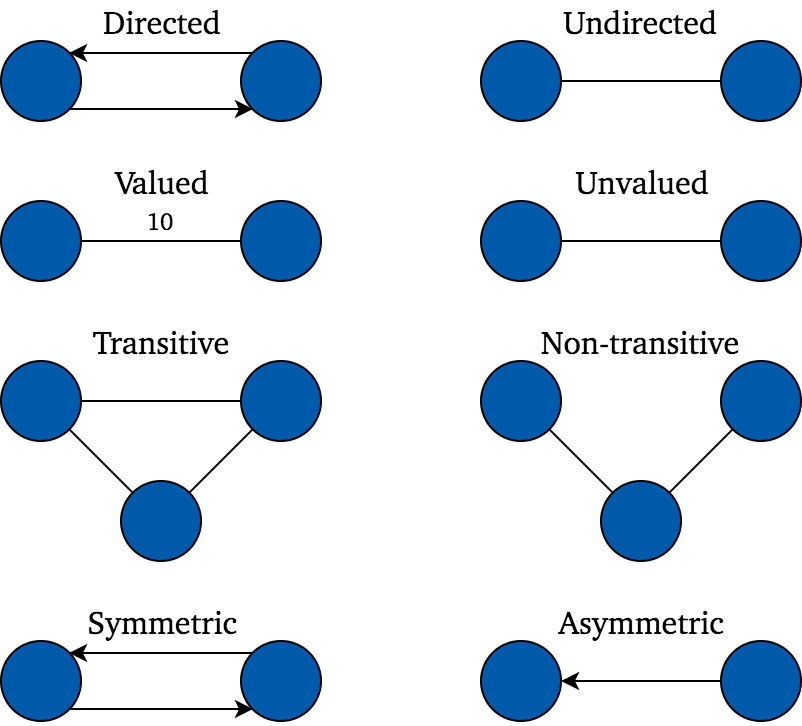
\includegraphics[height=8cm]{img/relation_properties}
  \caption{Relation properties in social networks}
\label{fig:tie_properties}
\end{figure}

Relations between actors can have several properties, as denoted in Fig.~\ref{fig:tie_properties}.
A first distinction has to be made between directed and undirected relations,
a property that also determines the directionality of the underlying graph.
An example for a directed relation would be resource transfers, an undirected
relation could be exemplified by marital relationships.
Relations can also be split into valued and unvalued types.
The attached value can stand for several properties, e.g., interaction intensity
between two actors.
Transitive relations occur when actor triples are connected to each other.
More intuitively, transitivity means that two related actors of an actor $n$ are
also related.
The final property exemplified in Fig.~\ref{fig:tie_properties} is symmetry which
is always given in undirected networks.
For directed networks, symmetry refers to the existence of a relation from
$n_i$ to $n_j$, if there is a relation in the opposite direction~\footcite{Wasserman1994}.

\paragraph{Properties}
\label{sub:sn_properties}

Social network analysis is a research area which examines dynamics in social
networks.
A central research question is the identification of important actors within
a network.
Important actors are also referred to as prestigious or prominent, where importance
represents the extent to which these actors are involved with others.
Here, involvement means being the sender or recipient of interactions in the
network.
A common measure for actor prominence is \textit{centrality}, which delivers
several characteristic numbers for measuring activity and location of an actor~\footcite{Wasserman1994}.
An important observation in social network research is the \textit{small world problem},
which is related to the probability of two random actors in a network being
connected to each other.
Formulated differently, the problem also comprises the question how many
mutual acquaintances are needed to form a path between these random actors.
Experiments lead to the conclusion that the distance between two actors in
a network is surprisingly low~\footcite{Travers1969}.
This gives way to observations that stress the importance of so-called
\textit{weak ties}, i.e., relations between actors that are less intense and
intimate, but serve significant roles in information diffusion~\footcite{Granovetter1973}.

\begin{figure}[h]
  
\includegraphics[height=6cm]{img/power_law_linkages}
  \caption[Power Law Distribution of Node Linkages]{Power Law Distribution of Node Linkages~\footcite{Barabasi2003}}
\label{fig:power_law}
\end{figure}

In addition to the small world phenomenon, many social networks are observed to
be \textit{scale-free}.
Scale freedom denotes the observation that few actors have a very high number of connections,
while the vast majority of actors is limited to very few connections.
Highly connected nodes are referred to as \textit{hubs}.
A power law distribution can be observed in scale-free networks, i.e., the
probability for an actor to have exactly $k$ connections is given by $k^{-n}$
where $n$ is approximately 2~\footcite{Barabasi2003}.
Fig.~\ref{fig:power_law} shows the power law distribution of node linkages both
on a regular and log-scale.

\paragraph{Social media}
\label{sub:sn_social_media}

The terms social network and social media are often used interchangeably, though
they generally refer to distinct matters.
Social media can be described as ``a group of Internet-based applications that
build on the ideological and technological foundations of Web 2.0, and that allow
the creation and exchange of User Generated Content''~\footcite[61]{Kaplan2010}.
Here, Web 2.0 refers to technologies like \textit{Flash}, \textit{RSS} and 
\textit{AJAX} that first enabled collaboration on the internet, e.g., via blogs
or wiki pages.
Examples for social media platforms are \textit{Facebook} (social network), 
\textit{Twitter} (microblogging) or \textit{YouTube} (video platform).
Rise of social media platforms brings practical challenges for organizations with it,
since they enable both direct communication with the customer, as well as
communication between customers.
Contents and frequency of the latter are mostly out of managerial control~\footcite{Mangold2009}.
Nowadays, most companies maintain social media profiles as part of their overall
marketing approach.
Research has created guidelines for corporate use of social media and stressed the
importance of community building around products of a company~\footcite{Culnan2010}.
Here, tracking the return of social media investments often requires engagement
statistics, e.g., number of followers, visits or replies, as well as community
sentiment~\footcite{Hoffman2010}.
Attributes of social media marketing have been shown to have positive effects
on purchase intention, e.g., for luxury fashion brands~\footcite{Kim2012}.

Twitter has been listed as an example social media platform.
The concluding section of this background chapter will explain terminology
and properties related to Twitter in more detail.


\subsubsection{Twitter}
\label{sub:sn_twitter}

Twitter is a microblogging service that enables its users to share short
messages with their followers.
The company was founded in 2006 and has grown to 330 million monthly active
users worldwide as of 2017.
Main revenue source for Twitter are advertisements which account for more than
85\% of revenue in 2017.
The last fiscal quarter of 2017 marked the first profitable period in Twitter
history, with profits equalling 91 million USD at a revenue of 732 million USD.
Here, video is the main advertisement format used on the platform~\footcite{Twitter2018}.
Twitter has also invested in live streaming events, e.g., football games~\footnote{\url{https://www.bloomberg.com/news/articles/2016-04-05/twitter-said-to-win-nfl-deal-for-thursday-night-streaming-rights}}.

Later parts of this thesis relate to specific Twitter terminology.
The most common terms will be presented in the following.
Users of the Twitter platform open an account with a unique user name (starting
with the ``@'' symbol).
Users can be verified by Twitter if their account is of public interest, e.g.,
for celebrities, companies or politicians~\footnote{\url{https://help.twitter.com/de/managing-your-account/about-twitter-verified-accounts}}.
If a user wants to receive updates from another user, he can follow his
account.
Relations between users are not necessarily symmetric, resulting in a distinction
between incoming and outgoing links.
Incoming relations,
i.e., being followed, are called ``followers'' and outgoing relations, i.e.,
following, are refered to as ``friends''.
Twitter allows curating users onto lists, which for example enables receiving topic-bound
status updates.
The number of lists a user is assigned to can be found in his account under the
term ``listings''.
Users publish short messages called ``tweets'', which can be seen in their user
account and appear in the timeline of followers.
Other users can engage with tweets through ``favorites'', ``retweets'' and ``replies''.
When sharing a tweet via a retweet, users have the option to add extra content.
If they opt for this approach, the resulting update is treated like a whole new
status message and referred to as a ``quote''~\footcite{Kwak2010}.
Quotes receive distinct engagement statistics, whereas engagement in retweets
is counted towards the original message.
The above described differentiation is important for later parts of this thesis.

This section about Twitter terminology completes the background chapter.
The next chapter will explain the general methodology used in this work.

